\documentclass{article}
% General
	\usepackage{graphicx} % Required for inserting images
	\setlength{\parindent}{0pt}
	\setlength{\parskip}{8pt} % Vertical space between paragraphs
	\setlength{\baselineskip}{18pt} % Vertical space between lines
	\usepackage{amsthm}
	\usepackage{mdframed}
	\usepackage{hyperref} % Add the hyperref package for clickable links
	\newcommand\bigO{\mathrm{O}}
	\usepackage[T1]{fontenc}


% Define the theorem-like environments
	% Define a new theorem style with upright text
	\newtheoremstyle{plainupright} % Name of the style
	{10pt}                        % Space above
	{3pt}                        % Space below
	{}                           % Body font (default is \itshape which is italics)
	{}                           % Indent amount
	{\bfseries}                  % Theorem head font
	{.}                          % Punctuation after theorem head
	{ }                          % Space after theorem head
	{}                           % Theorem head spec (can be left empty, meaning 'normal')
	
	\theoremstyle{plainupright}

	\newtheorem{theorem}{Theorem}[section]  % Numbering within sections
	\newtheorem{definition}[theorem]{Definition}  % Numbering with theorems
	\newtheorem{corollary}[theorem]{Corollary}  % Numbering with theorems
	\newtheorem{claim}[theorem]{Claim}  % Numbering with theorems
	\newtheorem{lemma}[theorem]{Lemma}  % Numbering with theorems
	\newtheorem{axiom}[theorem]{Axiom}  % Numbering with theorems
	\newtheorem{conjecture}[theorem]{Conjecture}  % Numbering with theorems
	\newtheorem{problem}[theorem]{Problem}  % Numbering with theorems

% Enclose theorem-like environments within boxes
	\surroundwithmdframed[style=theoremstyle]{theorem}
	\surroundwithmdframed[style=theoremstyle]{definition}
	\surroundwithmdframed[style=theoremstyle]{corollary}
	\surroundwithmdframed[style=theoremstyle]{claim}
	\surroundwithmdframed[style=theoremstyle]{lemma}
	\surroundwithmdframed[style=theoremstyle]{axiom}
	\surroundwithmdframed[style=theoremstyle]{conjecture}
	\surroundwithmdframed[style=theoremstyle]{problem}

% Define a box style for the theorem-like environments
	\mdfdefinestyle{theoremstyle}{%
		linewidth=0pt,
		backgroundcolor=white,
		roundcorner=5pt,
		innertopmargin=6pt,
		innerbottommargin=0pt,
		innerrightmargin=32pt,
		innerleftmargin=16pt,
	}	

% Set margins
	\usepackage{geometry}
	\geometry{
		left=3cm,
		right=3cm,
		top=2cm,
		bottom=2cm
	}

% Codeblock
	\usepackage{minted}
	\usepackage{xcolor}
	\definecolor{mintedBg}{rgb}{0.98,0.98,0.98}
	\setminted[py]{
		bgcolor=mintedBg,
		framesep=3mm,
		fontsize=\footnotesize,
		linenos,
		breaklines,
		breakanywhere,
	}
	\newcommand{\pyfile}[1]{%
		\textsf{%
			\detokenize{#1}%
		}%
		\par
		\inputminted{py}{../code/\detokenize{#1}}%
	}



\title{Implementation of a minimum branch-decomposition and branch-width algorithm for planar graphs.}
\author{Kristoffer Højelse}
\date{February 2024}

\begin{document}

\maketitle

% west https://dwest.web.illinois.edu/grammar.html
% The abstract states the results as fully as possible in a brief presentation. Crucial specialized terms the reader needs to know to understand the statements should be defined. The abstract stands on its own, especially in the age of electronic communication where it may be separate from the rest of the paper, and hence it contains no numbered reference to the bibliography.

\begin{abstract}
	Seymour and Thomas give an algorithm, the rat-catching algorithm, for deciding $bw(G) \leq c$ in $O(n^2)$ time, and by using it as a subroutine, an algorithm to compute an optimal branch-decomposition in $O(n^4)$ time. In this paper, I describe an implementation of this algorithm and publish the source code.
\end{abstract}

% The first section of the paper is an "Introduction" that should motivate the problem, discuss related results, state the results more completely, and perhaps summarize the techniques or the structure of the paper or crucial definitions.

\section{Introduction}

	In complexity theory, an NP-hard problem has no known algorithm with all 3 of these properties: (1) runs in polynomial time, (2) gives an exact solution, and (3) runs on all instances of the problem.

	You can find brute-force algorithms for NP-hard problems that both give an exact solution and run on all instances of the problem, but they run in exponential time.

	You can find approximation algorithms for NP-hard problems that both run in polynomial time and run on all instances, but they give an approximate solution.

	Finally, you can find parameterized algorithms for NP-hard problems that both run in polynomial time and give an exact solution, but they only run on instances of the problem where some parameter is small. Treewidth is a common such parameter.
	
	Treewidth is a measure of how tree-like a graph is, a value of 1 is exactly a tree and larger values are less tree-like. For some NP-hard problems, if a graph is sufficiently tree-like, then a parameterized algorithm can find an exact solution in polynomial time. For instance, the best-known running time for the \textsc{The Maximum Independent Set Problem} is exponential in $n$, particularly $O(1.1996^n \cdot n^{O(1)})$\cite{XN17}, but can be solved in $O(2^k \cdot k \cdot n)$ time for graphs of treewidth at most $k$, which is linear in $n$ and exponential in $k$.

	Branch width and carving width are related to treewidth, and some NP-hard problems can be solved efficiently for graphs of small branchwidth.\cite{CNP+11}

	Tree-, branch- and carving-width are all related. The treewidth of a graph is at least bw-1 and at most floor(3/2bw)-1.\cite{RS91}

	The carving width is at least half the branch width and is at most the degree times the branch width.\cite{ED18}

	You might have a parameterized algorithm with tree- or branch-width as a parameter, but to determine if a graph has a small tree- or branch-width, you might need to compute the tree- or branch-decomposition first. There is no known optimal tree decomposition/treewidth algorithm even for planar graphs.

	A planar graph is, informally, a graph that you can draw on a plane surface without any edges crossing. There might be multiple such drawings of a planar graph. A particular such drawing is called a plane graph.
	
	The algorithm by Seymour and Thomas\cite{ST93} computes a minimum branch-decomposition of a planar graph in $O(n^4)$ time.

	You can obtain an approximate optimum tree decomposition from the branch decomposition. So computing an approximate treewidth for planar graphs is possible in polynomial time.

	The concepts of medial graph and dual graph are used in the algorithm. Both are planar graphs, that are constructed from a plane graph.
	
	The dual graph has vertices for faces and edges connecting the faces that share an edge. You might imagine a map of countries, with edges for borders, and a vertex for each country, plus a vertex for the surrounding sea. You could for instance query such a network for which countries are neighbors, or which countries are landlocked.

	The medial graph also considers the faces but has vertices for edges, that are connected if the original edges were consecutive in some face. I have found no good metaphors for this.

	\todo{introduce seymour thomas contraction and rat-catching algorithm}

	Pino\cite{Pin16} applies branch decompositions.

	Seymour and Thomas\cite{ST93} give the rat-catching algorithm.

	Bian, Gu and Zhu\cite{BGZ15} describe and benchmark some implementations.

	\todo{Read params book about tree width}

\section{Preliminaries}

	This section defines the terms and concepts used in the algorithm.

	The algorithm deals with graphs that might have parallel edges. Distinguishing between two parallel edges is crucial. Therefore, the implementation gives labels to both vertices and edges, by encoding a graph as an adjacency list of edge IDs and a map from unique edge IDs to its vertex-pair.

	A \textit{graph} $G$ consists of a vertex set $V(G)$, and an edge set $\mathbb{E}(G)$ and a function $\phi_G$, where $V(G) \subset \mathbb{N}^+$ and where $\mathbb{E}(G) \subset \mathbb{N}^+$ and where $\phi_G \st \mathbb{E}(G) \to \{\{u,v\} \st u,v \in V(G)\}$.

	\textbf{Note.} Normally \textit{graph} refers to a simple graph, usually also without labels, which are normally encoded by an adjacency list or matrix. In this paper, a graph is a multigraph with labels.

	\textbf{Note.} Regarding notation, $V$ and $\mathbb{E}$ are operations on graphs returning the vertex set and edge set respectively.

	Let $E(G)$ return a multiset of all vertex-pairs of $G$; in other words, $E(G) = \{\phi_G(e) \st e \in \mathbb{E}(G)\}$.

	A \textit{drawing} of a graph $G$ is a node-link diagram in which the vertices are represented as disks and the edges are represented as line segments or curves in the Euclidean plane.

	Here is a drawing of a graph $G$.

	\begin{center}
		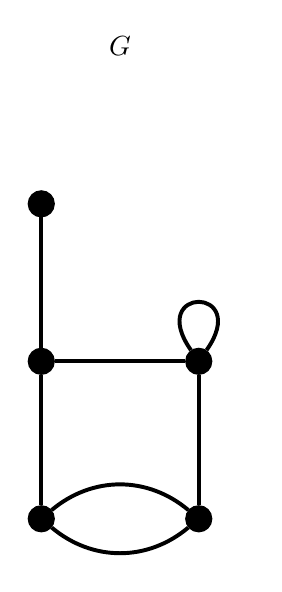
\begin{tikzpicture}
    \begin{scope}[xshift=0cm, yshift=0cm]
        \node (G) at (1, 6) {$G$};

        \node[circle, draw, fill=black, minimum size=0.01mm] (1) at (0, 4) {};
        \node[circle, draw, fill=black, minimum size=0.01mm] (2) at (0, 2) {};
        \node[circle, draw, fill=black, minimum size=0.01mm] (3) at (0, 0) {};
        \node[circle, draw, fill=black, minimum size=0.01mm] (4) at (2, 2) {};
        \node[circle, draw, fill=black, minimum size=0.01mm] (5) at (2, 0) {};

        % Draw the edges between nodes
        \draw[line width=0.5mm] (1) -- (2);
        \draw[line width=0.5mm] (2) -- (3);
        \draw[line width=0.5mm] (2) -- (4);
        \draw[line width=0.5mm] (4) -- (5);
        \draw[line width=0.5mm] (3) to[bend left=40] (5);
        \draw[line width=0.5mm] (3) to[bend right=40] (5);
        \draw[line width=0.5mm] (4) to[in=125,out=55,loop, min distance=1cm] (4);
    \end{scope}
\end{tikzpicture}

	\end{center}

	Here is a labeled drawing of the same graph $G$ and its function $\phi_G$.

	\begin{center}
		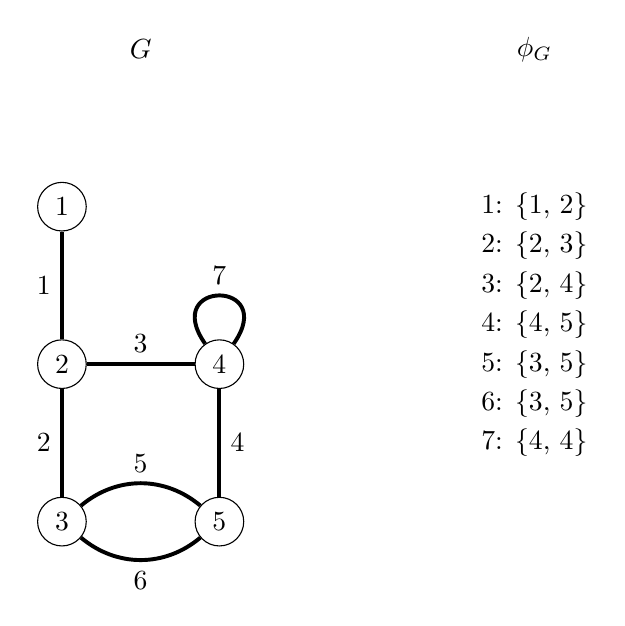
\begin{tikzpicture}
	% Define the nodes with specific positions
	\begin{scope}[xshift=0cm, yshift=0cm]
		\node (G) at (1, 6) {$G$};

		\node[circle, draw] (1) at (0, 4) {1};
		\node[circle, draw] (2) at (0, 2) {2};
		\node[circle, draw] (3) at (0, 0) {3};
		\node[circle, draw] (4) at (2, 2) {4};
		\node[circle, draw] (5) at (2, 0) {5};
	
		% Draw the edges between nodes with labels
		\draw[line width=0.5mm] (1) -- node[left] {1} (2);
		\draw[line width=0.5mm] (2) -- node[left] {2} (3);
		\draw[line width=0.5mm] (2) -- node[above] {3} (4);
		\draw[line width=0.5mm] (4) -- node[right] {4} (5);
		\draw[line width=0.5mm] (3) to[bend left=40] node[above] {5} (5);
		\draw[line width=0.5mm] (3) to[bend right=40] node[below] {6} (5);
		\draw[line width=0.5mm] (4) to[in=125,out=55,loop, min distance=1cm] node[above] {7} (4);
	\end{scope}

	% Draw the mapping from edge IDs to vertex pairs
	\begin{scope}[xshift=6cm, yshift=0cm]
		\node (E0) at (0, 6) {$\phi_G$};
		\node (E1) at (0, 4) {1: \{1, 2\}};
		\node (E2) at (0, 3.5) {2: \{2, 3\}};
		\node (E3) at (0, 3) {3: \{2, 4\}};
		\node (E4) at (0, 2.5) {4: \{4, 5\}};
		\node (E5) at (0, 2) {5: \{3, 5\}};
		\node (E6) at (0, 1.5) {6: \{3, 5\}};
		\node (E7) at (0, 1) {7: \{4, 4\}};
	\end{scope}
\end{tikzpicture}
	\end{center}

	A \textit{self-loop}, is an edge $e$ where $\phi_G(e) = \{u,v\}$ and $u = v$.

	A graph $G$ is \textit{loop-less}, if no edge $e \in \mathbb{E}(G)$ is a self-loop. The edge with label 7, in the graph above, is an example of a self-loop.

	A graph $G$ is \textit{simple}, if it has no parallel edges; in other words, if all elements of $E(G)$ are pair-wise distinct.

	\begin{center}
		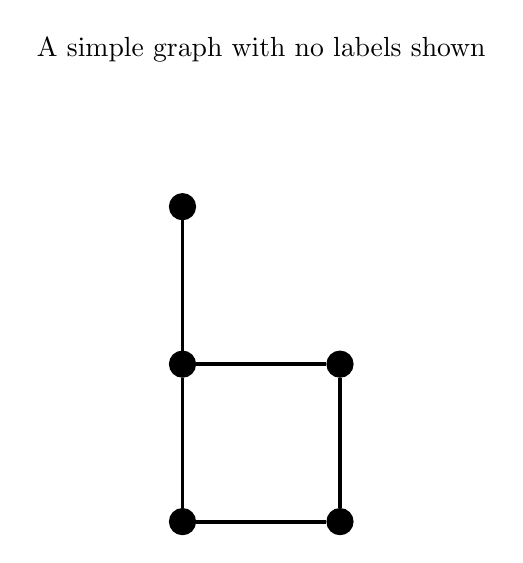
\begin{tikzpicture}
    % Define the nodes with specific positions
    \begin{scope}[xshift=0cm, yshift=0cm]
        \node (G) at (1, 6) {A simple graph with no labels shown};

        \node[circle, draw, fill=black, minimum size=0.01mm] (1) at (0, 4) {};
        \node[circle, draw, fill=black, minimum size=0.01mm] (2) at (0, 2) {};
        \node[circle, draw, fill=black, minimum size=0.01mm] (3) at (0, 0) {};
        \node[circle, draw, fill=black, minimum size=0.01mm] (4) at (2, 2) {};
        \node[circle, draw, fill=black, minimum size=0.01mm] (5) at (2, 0) {};

        % Draw the edges between nodes
        \draw[line width=0.5mm] (1) -- (2);
        \draw[line width=0.5mm] (2) -- (3);
        \draw[line width=0.5mm] (2) -- (4);
        \draw[line width=0.5mm] (4) -- (5);
        \draw[line width=0.5mm] (3) -- (5);
    \end{scope}
\end{tikzpicture}

	\end{center}

	A \textit{subgraph} $H$ of a graph $G$, is a graph where some vertices and edges might be missing; in other words, is a graph where $V(H) \subseteq V(G)$ and where $\mathbb{E}(H) \subseteq \mathbb{E}(G)$ and where $\forall e \in \mathbb{E}(H), \phi_H(e) = \phi_G(e)$.

	\begin{center}
		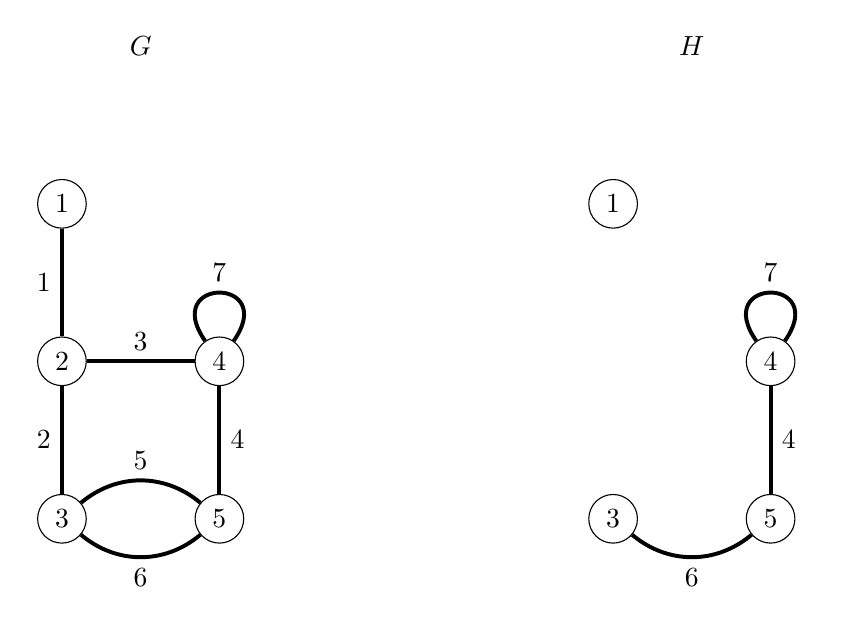
\begin{tikzpicture}
	\begin{scope}[xshift=0cm, yshift=0cm]
		\node (G) at (1, 6) {$G$};

		\node[circle, draw] (1) at (0, 4) {1};
		\node[circle, draw] (2) at (0, 2) {2};
		\node[circle, draw] (3) at (0, 0) {3};
		\node[circle, draw] (4) at (2, 2) {4};
		\node[circle, draw] (5) at (2, 0) {5};
	
		% Draw the edges between nodes with labels
		\draw[line width=0.5mm] (1) -- node[left] {1} (2);
		\draw[line width=0.5mm] (2) -- node[left] {2} (3);
		\draw[line width=0.5mm] (2) -- node[above] {3} (4);
		\draw[line width=0.5mm] (4) -- node[right] {4} (5);
		\draw[line width=0.5mm] (3) to[bend left=40] node[above] {5} (5);
		\draw[line width=0.5mm] (3) to[bend right=40] node[below] {6} (5);
		\draw[line width=0.5mm] (4) to[in=125,out=55,loop, min distance=1cm] node[above] {7} (4);
	\end{scope}

	\begin{scope}[xshift=7cm, yshift=0cm]
		\node (G) at (1, 6) {$H$};

		\node[circle, draw] (1) at (0, 4) {1};
		\node[circle, draw] (3) at (0, 0) {3};
		\node[circle, draw] (4) at (2, 2) {4};
		\node[circle, draw] (5) at (2, 0) {5};
	
		% Draw the edges between nodes with labels
		\draw[line width=0.5mm] (4) -- node[right] {4} (5);
		\draw[line width=0.5mm] (3) to[bend right=40] node[below] {6} (5);
		\draw[line width=0.5mm] (4) to[in=125,out=55,loop, min distance=1cm] node[above] {7} (4);
	\end{scope}
\end{tikzpicture}

	\end{center}

	For $A \subseteq V(G)$, we denote by $G[A]$ the subgraph induced by the subset of vertices $A$; in other words, $G[A]$ is the subgraph where $V(G[A]) = A$ and where $\mathbb{E}(G[A]) = \{ e \st e \in \mathbb{E}(G) \land |\phi_G(e) \cap A| = 2\}$ and where $\forall e \in E(G[A]), \phi_{G[A]}(e) = \phi_{G}(e)$.

	\begin{center}
		\begin{tikzpicture}
	\begin{scope}[xshift=0cm, yshift=0cm]
		\node (G) at (1, 6) {$G$};

		\node[circle, draw] (1) at (0, 4) {1};
		\node[circle, draw] (2) at (0, 2) {2};
		\node[circle, draw] (3) at (0, 0) {3};
		\node[circle, draw] (4) at (2, 2) {4};
		\node[circle, draw] (5) at (2, 0) {5};
	
		% Draw the edges between nodes with labels
		\draw[line width=0.5mm] (1) -- node[above] {1} (2);
		\draw[line width=0.5mm] (2) -- node[left] {2} (3);
		\draw[line width=0.5mm] (2) -- node[above] {3} (4);
		\draw[line width=0.5mm] (4) -- node[right] {4} (5);
		\draw[line width=0.5mm] (3) to[bend left=40] node[above] {5} (5);
		\draw[line width=0.5mm] (3) to[bend right=40] node[below] {6} (5);
		\draw[line width=0.5mm] (4) to[in=125,out=55,loop, min distance=1cm] node[above] {7} (4);
	\end{scope}
	
	\begin{scope}[xshift=6cm, yshift=0cm]
		\node (E0) at (0, 6) {$A$};
		\node (E1) at (0, 4) {\{1, 3, 4, 5\}};
	\end{scope}

	\begin{scope}[xshift=10cm, yshift=0cm]
		\node (G) at (1, 6) {$G[A]$};

		\node[circle, draw] (1) at (0, 4) {1};
		\node[circle, draw] (3) at (0, 0) {3};
		\node[circle, draw] (4) at (2, 2) {4};
		\node[circle, draw] (5) at (2, 0) {5};
	
		% Draw the edges between nodes with labels
		\draw[line width=0.5mm] (4) -- node[right] {4} (5);
		\draw[line width=0.5mm] (3) to[bend left=40] node[above] {5} (5);
		\draw[line width=0.5mm] (3) to[bend right=40] node[below] {6} (5);
		\draw[line width=0.5mm] (4) to[in=125,out=55,loop, min distance=1cm] node[above] {7} (4);
	\end{scope}
\end{tikzpicture}

	\end{center}

	A vertex $v \in V(G)$ and an edge $e \in \mathbb{E}(G)$ are \textit{incident} to each other, if $v \in \phi_G(e)$. Furthermore, two distinct edges $e_1,e_2 \in \mathbb{E}(G)$ are incident to each other, if $\phi_G(e_1) \cap \phi_G(e_2) \neq \emptyset$.

	The \textit{degree} of a vertex $v$, denoted $\deg(v)$, is the number of times that an edge is incident to $v$. A self-loop is incident to the same vertex twice.

	\begin{center}
		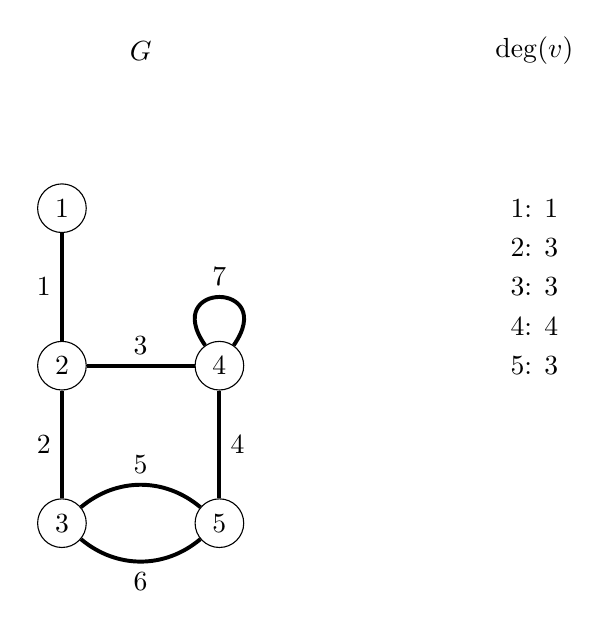
\begin{tikzpicture}
	% Define the nodes with specific positions
	\begin{scope}[xshift=0cm, yshift=0cm]
		\node (G) at (1, 6) {$G$};

		\node[circle, draw] (1) at (0, 4) {1};
		\node[circle, draw] (2) at (0, 2) {2};
		\node[circle, draw] (3) at (0, 0) {3};
		\node[circle, draw] (4) at (2, 2) {4};
		\node[circle, draw] (5) at (2, 0) {5};
	
		% Draw the edges between nodes with labels
		\draw[line width=0.5mm] (1) -- node[left] {1} (2);
		\draw[line width=0.5mm] (2) -- node[left] {2} (3);
		\draw[line width=0.5mm] (2) -- node[above] {3} (4);
		\draw[line width=0.5mm] (4) -- node[right] {4} (5);
		\draw[line width=0.5mm] (3) to[bend left=40] node[above] {5} (5);
		\draw[line width=0.5mm] (3) to[bend right=40] node[below] {6} (5);
		\draw[line width=0.5mm] (4) to[in=125,out=55,loop, min distance=1cm] node[above] {7} (4);
	\end{scope}

	% Draw the mapping from edge IDs to vertex pairs
	\begin{scope}[xshift=6cm, yshift=0cm]
		\node (E0) at (0, 6) {$\deg(v)$};
		\node (E1) at (0, 4) {1: 1};
		\node (E2) at (0, 3.5) {2: 3};
		\node (E3) at (0, 3) {3: 3};
		\node (E4) at (0, 2.5) {4: 4};
		\node (E5) at (0, 2) {5: 3};
	\end{scope}
\end{tikzpicture}
	\end{center}

	The \textit{maximum degree} of a graph $G$, denoted $\Delta(G)$, is the maximal degree of any vertex of $G$.

	$$\Delta(G) = 4$$

	A \textit{walk} of a graph $G$ is a list $[v_0,e_1,v_1,...,e_k,v_k]$ where $v_0,v_1,...,v_k \in V(G)$ and for $1 \leq i \leq k$, $\phi_{G}(e_i) = \{v_{i-1}, v_i\}$.

	A walk of $G$ $$[4,7,4,4,5,5,3,5,5,6,3]$$

	The \textit{length} of a walk is the number of edges in the walk.
	
	An \textit{s,t-walk} is a walk where $s = v_0$ and $t = v_k$.

	An $s,t$-walk is \textit{closed}, if $s = t$.

	A \textit{path} of a graph $G$, is a walk such that no vertex is repeated in the list.

	A \textit{cycle} of a graph $G$, is an $s,t$-walk such that no vertex is repeated in the list except $s=t$.

	A graph $G$ is \textit{connected} if there exists a $s,t$-walk for every pair of distinct vertices $s,t \in V(G)$.

	A \textit{component} of a graph, is a connected subgraph.

	A \textit{bijection} (or \textit{one-to-one correspondence}) is a relation between two sets such that each element of either set is paired with exactly one element of the other set.

	A \textit{plane graph} is a drawing of a graph, such that no edges are crossing.
	
	A graph $G$ is \textit{planar}, if there exists a \textit{plane graph} of $G$.

	A \textit{rotation system} is an encoding of a graph, in particular, it is an adjacency list such that the neighborhood, around any vertex, is in clockwise ordering according to some plane embedding of $G$.

	\begin{definition}\label{def:contraction}
		(\textit{Contraction})

		A contraction is a function that given a multi-graph (with no self-loops) $G$ and pair of distinct vertices $u,v$ of some edge $\{u,v\} \in E(G)$, removes $e$ if $\phi_G(e) = \{u,v\}$ and makes any edge that is adjacent to $v$, $\phi_G(e) = \{w,v\}$, adjacent to $u$ instead, $\phi_G(e) = \{w,u\}$, and finally returns the resulting graph.
	\end{definition}

	\begin{corollary}
		The resulting graph of a contraction will not have any self-loops.
	\end{corollary}

	\begin{center}
		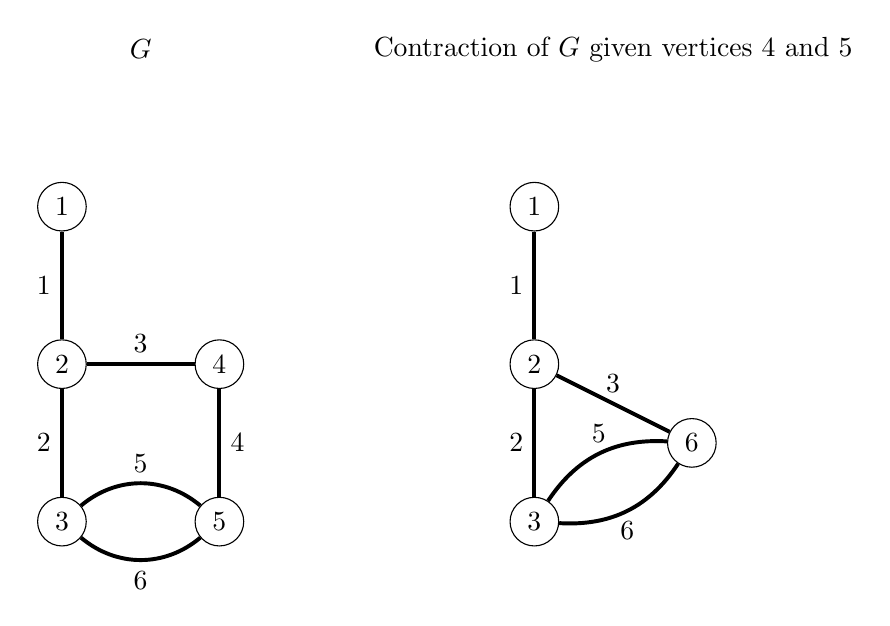
\begin{tikzpicture}
	\begin{scope}[xshift=0cm, yshift=0cm]
		\node (G) at (1, 6) {$G$};

		\node[circle, draw] (1) at (0, 4) {1};
		\node[circle, draw] (2) at (0, 2) {2};
		\node[circle, draw] (3) at (0, 0) {3};
		\node[circle, draw] (4) at (2, 2) {4};
		\node[circle, draw] (5) at (2, 0) {5};
	
		% Draw the edges between nodes with labels
		\draw[line width=0.5mm] (1) -- node[left] {1} (2);
		\draw[line width=0.5mm] (2) -- node[left] {2} (3);
		\draw[line width=0.5mm] (2) -- node[above] {3} (4);
		\draw[line width=0.5mm] (4) -- node[right] {4} (5);
		\draw[line width=0.5mm] (3) to[bend left=40] node[above] {5} (5);
		\draw[line width=0.5mm] (3) to[bend right=40] node[below] {6} (5);
	\end{scope}
	
	\begin{scope}[xshift=6cm, yshift=0cm]
		\node (G) at (1, 6) {Contraction of $G$ given vertices 4 and 5};

		\node[circle, draw] (1) at (0, 4) {1};
		\node[circle, draw] (2) at (0, 2) {2};
		\node[circle, draw] (3) at (0, 0) {3};
		\node[circle, draw] (6) at (2, 1) {6};
	
		% Draw the edges between nodes with labels
		\draw[line width=0.5mm] (1) -- node[left] {1} (2);
		\draw[line width=0.5mm] (2) -- node[left] {2} (3);
		\draw[line width=0.5mm] (2) -- node[above] {3} (6);
		\draw[line width=0.5mm] (3) to[bend left=30] node[above] {5} (6);
		\draw[line width=0.5mm] (3) to[bend right=30] node[below] {6} (6);
	\end{scope}
\end{tikzpicture}

	\end{center}
	
	\begin{definition}\label{def:medial}
		(\textit{Medial Graph})
		
		The medial graph $G^\times$ of a connected plane graph $G$ is a graph such that there is a bijection between $V(G^\times)$ and $\mathbb{E}(G)$ and such that for each face $f$ of $G$, there's an edge $e^\times \in \mathbb{E}(G^\times)$ incident to a pair of vertices $u^\times,v^\times \in V(G^\times)$ if edges $u,v \in \mathbb{E}(G)$ are consecutive in $f$.
	\end{definition}

	\begin{center}
		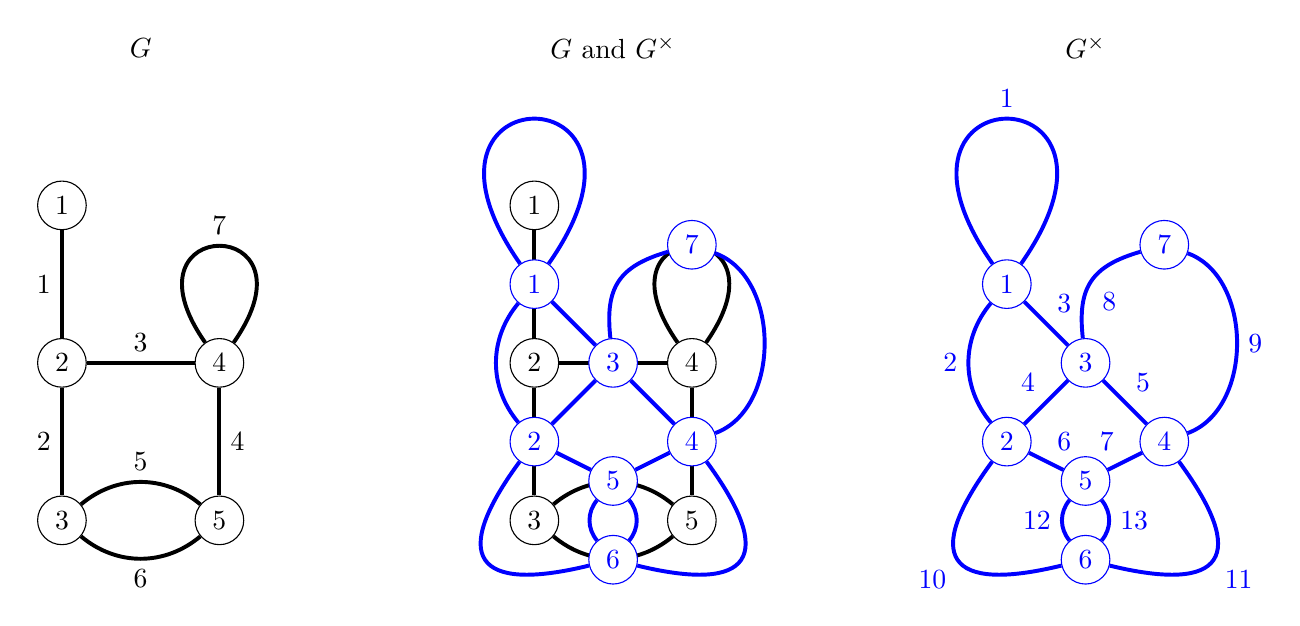
\begin{tikzpicture}
	\begin{scope}[xshift=0cm, yshift=0cm]
		\node (G) at (1, 6) {$G$};

		\node[circle, draw] (a1) at (0, 4) {1};
		\node[circle, draw] (a2) at (0, 2) {2};
		\node[circle, draw] (a3) at (0, 0) {3};
		\node[circle, draw] (a4) at (2, 2) {4};
		\node[circle, draw] (a5) at (2, 0) {5};
	
		% Draw the edges between nodes with labels
		\draw[line width=0.5mm] (a1) -- node[left] {1} (a2);
		\draw[line width=0.5mm] (a2) -- node[left] {2} (a3);
		\draw[line width=0.5mm] (a2) -- node[above] {3} (a4);
		\draw[line width=0.5mm] (a4) -- node[right] {4} (a5);
		\draw[line width=0.5mm] (a3) to[bend left=40] node[above] {5} (a5);
		\draw[line width=0.5mm] (a3) to[bend right=40] node[below] {6} (a5);
		\draw[line width=0.5mm] (a4) to[in=125,out=55,loop, min distance=2cm] node[above] {7} (a4);
	\end{scope}

	\begin{scope}[xshift=6cm, yshift=0cm]
		\node (G) at (1, 6) {$G$ and $G^\times$};

		\node[circle, draw] (a1) at (0, 4) {1};
		\node[circle, draw] (a2) at (0, 2) {2};
		\node[circle, draw] (a3) at (0, 0) {3};
		\node[circle, draw] (a4) at (2, 2) {4};
		\node[circle, draw] (a5) at (2, 0) {5};
	
		% Draw the edges between nodes with labels
		\draw[line width=0.5mm] (a1) -- (a2);
		\draw[line width=0.5mm] (a2) -- (a3);
		\draw[line width=0.5mm] (a2) -- (a4);
		\draw[line width=0.5mm] (a4) -- (a5);
		\draw[line width=0.5mm] (a3) to[bend left=40] (a5);
		\draw[line width=0.5mm] (a3) to[bend right=40] (a5);
		\draw[line width=0.5mm] (a4) to[in=125,out=55,loop, min distance=2cm] (a4);

		\node[circle, draw, color=blue, fill=white] (b1) at (0, 3) {1};
		\node[circle, draw, color=blue, fill=white] (b2) at (0, 1) {2};
		\node[circle, draw, color=blue, fill=white] (b3) at (1, 2) {3};
		\node[circle, draw, color=blue, fill=white] (b4) at (2, 1) {4};
		\node[circle, draw, color=blue, fill=white] (b5) at (1, 0.5) {5};
		\node[circle, draw, color=blue, fill=white] (b6) at (1, -0.5) {6};
		\node[circle, draw, color=blue, fill=white] (b7) at (2, 3.5) {7};
	
		% Draw the edges between nodes with labels
		\draw[line width=0.5mm, color=blue] (b1) to[in=125,out=55,loop, min distance=3cm] (b1);
		\draw[line width=0.5mm, color=blue] (b1) to[bend right=40, min distance=0.5cm] (b2);
		\draw[line width=0.5mm, color=blue] (b1) -- (b3);
		\draw[line width=0.5mm, color=blue] (b2) -- (b3);
		\draw[line width=0.5mm, color=blue] (b3) -- (b4);
		\draw[line width=0.5mm, color=blue] (b2) -- (b5);
		\draw[line width=0.5mm, color=blue] (b5) -- (b4);
		\draw[line width=0.5mm, color=blue] (b3) to[bend left=40, min distance=0.65cm] (b7);
		\draw[line width=0.5mm, color=blue] (b4) to[bend right=70, min distance=0.5cm] (b7);
		\draw[line width=0.5mm, color=blue] (b2) to[bend right=70, min distance=1.5cm] (b6);
		\draw[line width=0.5mm, color=blue] (b4) to[bend left=70, min distance=1.5cm] (b6);
		\draw[line width=0.5mm, color=blue] (b5) to[bend right=40] (b6);
		\draw[line width=0.5mm, color=blue] (b5) to[bend left=40] (b6);
	\end{scope}

	\begin{scope}[xshift=12cm, yshift=0cm]
		\node (G) at (1, 6) {$G^\times$};

		\node[circle, draw, color=blue, fill=white] (b1) at (0, 3) {1};
		\node[circle, draw, color=blue, fill=white] (b2) at (0, 1) {2};
		\node[circle, draw, color=blue, fill=white] (b3) at (1, 2) {3};
		\node[circle, draw, color=blue, fill=white] (b4) at (2, 1) {4};
		\node[circle, draw, color=blue, fill=white] (b5) at (1, 0.5) {5};
		\node[circle, draw, color=blue, fill=white] (b6) at (1, -0.5) {6};
		\node[circle, draw, color=blue, fill=white] (b7) at (2, 3.5) {7};
	
		% Draw the edges between nodes with labels
		\draw[line width=0.5mm, color=blue] (b1) to[in=125,out=55,loop, min distance=3cm] node[above] {1} (b1);
		\draw[line width=0.5mm, color=blue] (b1) to[bend right=40, min distance=0.5cm] node[left] {2} (b2);
		\draw[line width=0.5mm, color=blue] (b1) -- node[above right] {3} (b3);
		\draw[line width=0.5mm, color=blue] (b2) -- node[above left] {4} (b3);
		\draw[line width=0.5mm, color=blue] (b3) -- node[above right] {5} (b4);
		\draw[line width=0.5mm, color=blue] (b2) -- node[above right] {6} (b5);
		\draw[line width=0.5mm, color=blue] (b5) -- node[above left] {7} (b4);
		\draw[line width=0.5mm, color=blue] (b3) to[bend left=40, min distance=0.65cm] node[below right] {8} (b7);
		\draw[line width=0.5mm, color=blue] (b4) to[bend right=70, min distance=0.5cm] node[right] {9} (b7);
		\draw[line width=0.5mm, color=blue] (b2) to[bend right=70, min distance=1.5cm] node[below left] {10} (b6);
		\draw[line width=0.5mm, color=blue] (b4) to[bend left=70, min distance=1.5cm] node[below right] {11} (b6);
		\draw[line width=0.5mm, color=blue] (b5) to[bend right=40] node[left] {12} (b6);
		\draw[line width=0.5mm, color=blue] (b5) to[bend left=40] node[right] {13} (b6);
	\end{scope}
\end{tikzpicture}

	\end{center}
	
	\begin{corollary}
		A medial graph is a 4-regular plane graph.
	\end{corollary}

	I will refer to vertices and edges of the medial graph as "nodes" and "links" in an attempt at disambiguation.

	\begin{definition}
		(\textit{Dual Graph})

		The dual graph $G^*$ of a plane graph $G$ is a graph with a bijection between the set of faces of $G$ and $V(G^*)$ and a bijection between $\mathbb{E}(G)$ and $\mathbb{E}(G^*)$ such that an edge $e \in \mathbb{E}(G)$ that separates two faces $f_1$,$f_2$ of $G$ is an edge $e^* \in \mathbb{E}(G^*)$ incident to $f_1^*$ and $f_2^*$.
	\end{definition}

	\begin{center}
		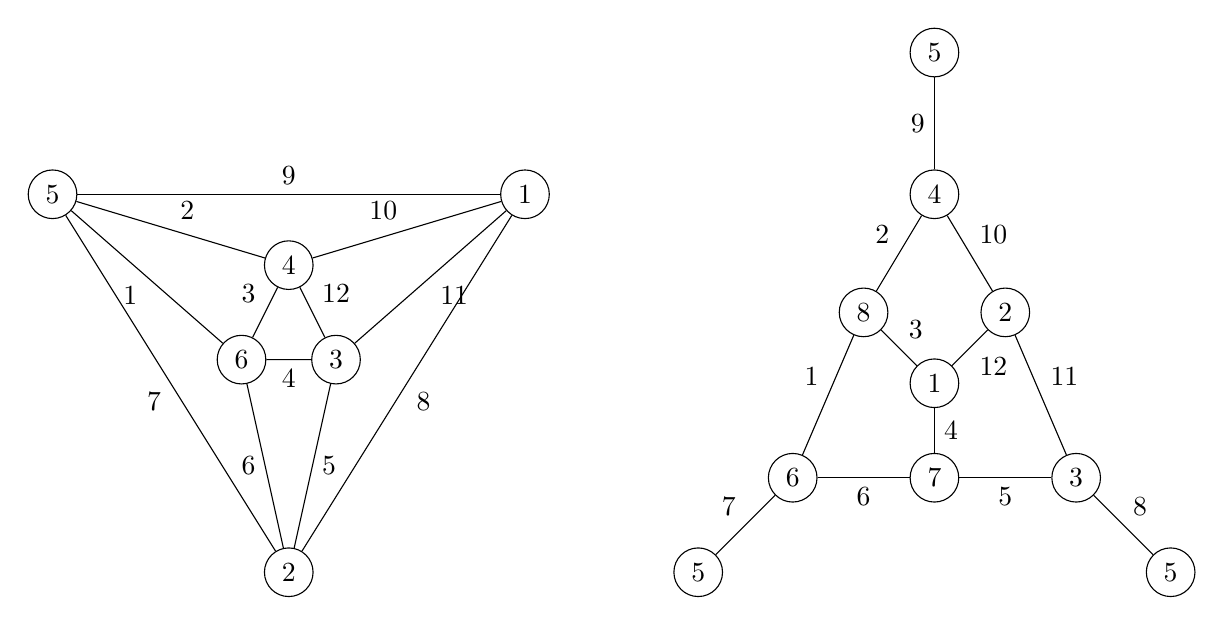
\begin{tikzpicture}
	% Define the nodes with specific positions
	\begin{scope}[xshift=0cm, yshift=0cm, scale=0.6]
		\node[circle, draw] (1) at (8, -0) {1};
		\node[circle, draw] (2) at (3, -8) {2};
		\node[circle, draw] (3) at (4, -3.5) {3};
		\node[circle, draw] (4) at (3, -1.5) {4};
		\node[circle, draw] (5) at (-2, -0) {5};
		\node[circle, draw] (6) at (2, -3.5) {6};
	
		% Draw the edges between nodes with labels
		\draw[draw] (5) -- node[below left] {1} (6);
		\draw[draw] (5) -- node[above right] {2} (4);
		\draw[draw] (4) -- node[above left] {3} (6);
		\draw[draw] (3) -- node[below] {4} (6);
		\draw[draw] (3) -- node[right] {5} (2);
		\draw[draw] (6) -- node[left] {6} (2);
		\draw[draw] (2) -- node[below left] {7} (5);
		\draw[draw] (1) -- node[below right] {8} (2);
		\draw[draw] (1) -- node[above] {9} (5);
		\draw[draw] (1) -- node[above left] {10} (4);
		\draw[draw] (1) -- node[below right] {11} (3);
		\draw[draw] (4) -- node[above right] {12} (3);
	\end{scope}

	\begin{scope}[xshift=10cm, yshift=-2.4cm, scale=0.6]
		\node[circle, draw] (d1) at (0, 0) {1};
		\node[circle, draw] (d2) at (1.5, 1.5) {2};
		\node[circle, draw] (d3) at (3, -2) {3};
		\node[circle, draw] (d4) at (0, 4) {4};
		\node[circle, draw] (d51) at (0, 7) {5};
		\node[circle, draw] (d52) at (5, -4) {5};
		\node[circle, draw] (d53) at (-5, -4) {5};
		\node[circle, draw] (d6) at (-3, -2) {6};
		\node[circle, draw] (d7) at (0, -2) {7};
		\node[circle, draw] (d8) at (-1.5, 1.5) {8};
	
		% Draw the edges between nodes with labels
		\draw[draw] (d6) -- node[above left] {1} (d8);
		\draw[draw] (d4) -- node[above left] {2} (d8);
		\draw[draw] (d1) -- node[above right] {3} (d8);
		\draw[draw] (d7) -- node[right] {4} (d1);
		\draw[draw] (d7) -- node[below] {5} (d3);
		\draw[draw] (d6) -- node[below] {6} (d7);
		\draw[draw] (d6) -- node[above left] {7} (d53);
		\draw[draw] (d3) -- node[above right] {8} (d52);
		\draw[draw] (d51) -- node[left] {9} (d4);
		\draw[draw] (d4) -- node[above right] {10} (d2);
		\draw[draw] (d2) -- node[above right] {11} (d3);
		\draw[draw] (d1) -- node[below right] {12} (d2);
	\end{scope}
\end{tikzpicture}
	\end{center}

	A \textit{tree} is a connected graph with no cycles.

	A \textit{leaf} $v$ of a tree $T$, is a vertex $v \in V(T)$ of degree 1.

	Let the \textit{leaf set} of a tree $T$, denoted $L(T)$, be the subset of vertices $L(T) \subseteq V(T)$ that are also leaves of $T$.
	
	An \textit{internal vertex} $v$ of a tree $T$, is a vertex $v \in V(T) - L(T)$ that is not a leaf. An internal vertex therefore has at least degree 2.

	An \textit{unrooted binary tree} $T$, is a tree where every internal vertex has degree 3.

	A \textit{Branch Decomposition} $(B_G, \delta_G)$ of a simple graph $G$ consists of firstly, an unrooted binary tree $B_G$ and secondly a bijection $\delta_G$ between $\mathbb{E}(G)$ and $L(B_G)$.

	Removing any edge $e \in \mathbb{E}(B_G)$ partitions $B_G$ into 2 trees $P_e$ and $Q_e$. The set $\cup\{\phi_G(e) \st e \in L(P_e)\} \cap \cup\{\phi_G(e) \st e \in L(Q_e)\}$ is called a \textit{middle set} of $B_G$ given $e$, denoted $Z(B_G,e)$. The maximal cardinality of any middle set of $B_G$ given any $e \in \mathbb{E}(B_G)$ is the width of $B_G$; in other words, the width of $B_G$ is $\max\{ |Z(B, e)| \st e \in \mathbb{E}(B) \}$.

	\todo{middle set definition is convoluted}

	A \textit{Minimum Branch Decomposition} of $G$ is any branch decomposition of $G$ of minimum width among all branch decompositions of $G$, as there might exist many branch decompositions of a graph $G$.

	\begin{center}
		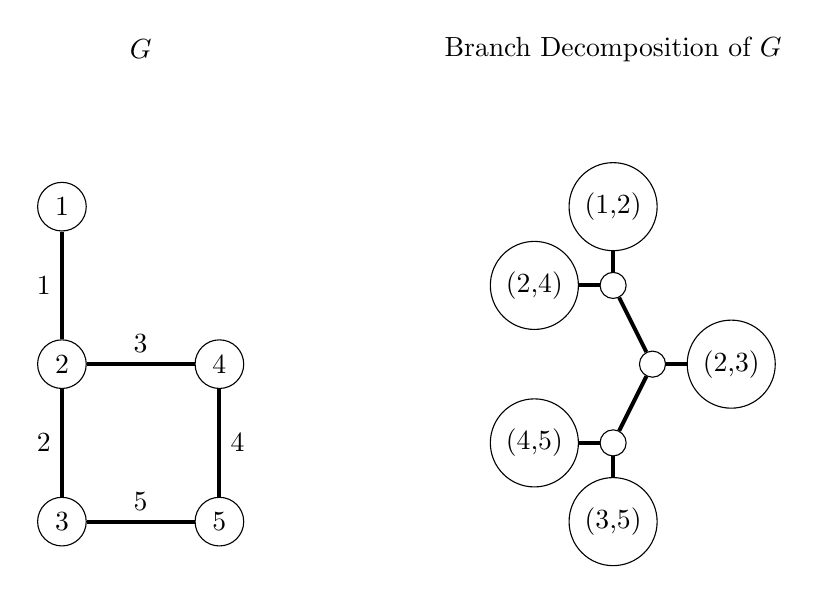
\begin{tikzpicture}
	\begin{scope}[xshift=0cm, yshift=0cm]
		\node (G) at (1, 6) {$G$};

		\node[circle, draw] (a1) at (0, 4) {1};
		\node[circle, draw] (a2) at (0, 2) {2};
		\node[circle, draw] (a3) at (0, 0) {3};
		\node[circle, draw] (a4) at (2, 2) {4};
		\node[circle, draw] (a5) at (2, 0) {5};
	
		% Draw the edges between nodes with labels
		\draw[line width=0.5mm] (a1) -- node[left] {1} (a2);
		\draw[line width=0.5mm] (a2) -- node[left] {2} (a3);
		\draw[line width=0.5mm] (a2) -- node[above] {3} (a4);
		\draw[line width=0.5mm] (a4) -- node[right] {4} (a5);
		\draw[line width=0.5mm] (a3) -- node[above] {5} (a5);
	\end{scope}

	\begin{scope}[xshift=6cm, yshift=0cm]
		\node (G) at (1, 6) {Branch Decomposition of $G$};

		\node[circle, draw, color=black, fill=white] (b1) at (1, 4) {(1,2)};
		\node[circle, draw, color=black, fill=white] (b3) at (0, 3) {(2,4)};
		\node[circle, draw, color=black, fill=white] (i1) at (1, 3) {};
		\node[circle, draw, color=black, fill=white] (i2) at (1.5, 2) {};
		\node[circle, draw, color=black, fill=white] (i3) at (1, 1) {};
		\node[circle, draw, color=black, fill=white] (b2) at (2.5, 2) {(2,3)};
		\node[circle, draw, color=black, fill=white] (b4) at (0, 1) {(4,5)};
		\node[circle, draw, color=black, fill=white] (b5) at (1, 0) {(3,5)};
	
		% Draw the edges between nodes with labels
		\draw[line width=0.5mm, color=black] (b1) -- (i1);
		\draw[line width=0.5mm, color=black] (b3) -- (i1);
		\draw[line width=0.5mm, color=black] (i1) -- (i2);
		\draw[line width=0.5mm, color=black] (b2) -- (i2);
		\draw[line width=0.5mm, color=black] (i2) -- (i3);
		\draw[line width=0.5mm, color=black] (i3) -- (b4);
		\draw[line width=0.5mm, color=black] (i3) -- (b5);
	\end{scope}
\end{tikzpicture}

	\end{center}

	A \textit{Carving Decomposition} $(C_G, \lambda_G)$ of a simple graph $G$ consists of firstly, an unrooted binary tree $C_G$ and secondly a bijection $\lambda_G$ between $V(G)$ and $L(C_G)$.

	Removing any edge $e \in \mathbb{E}(C_G)$ partitions $C_G$ into 2 trees $P_e$ and $Q_e$. The set of edges $e \in \mathbb{E}(G)$ that cross $L(P_e)$ and $L(Q_e)$ is called a \textit{crossing set} of $C_G$ given an $e \in \mathbb{E}(C_G)$, denoted $Y(C_G,e)$. The maximum cardinality of any crossing set of $C_G$ given any $e \in \mathbb{E}(C_G)$ is the width of $C_G$; in other words, the width of $C_G$ is $\max\{ |Y(C, e)| \st e \in \mathbb{E}(C) \}$.

	A \textit{Minimum Carving Decomposition} of $G$ is any carving decomposition of $G$ of minimum width among all carving decompositions of $G$, as there might exist many carving decompositions of a graph $G$.

	\begin{center}
		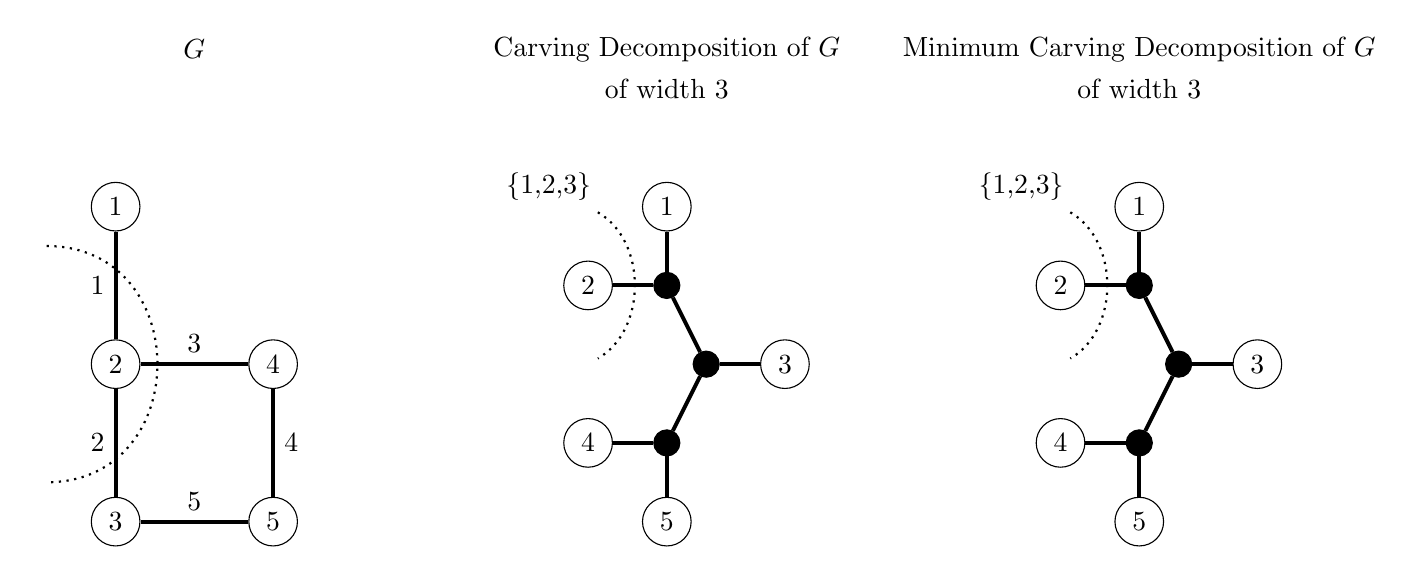
\begin{tikzpicture}
	\begin{scope}[xshift=0cm, yshift=0cm]
		\node (G) at (1, 6) {$G$};

		\node[circle, draw] (a1) at (0, 4) {1};
		\node[circle, draw] (a2) at (0, 2) {2};
		\node[circle, draw] (a3) at (0, 0) {3};
		\node[circle, draw] (a4) at (2, 2) {4};
		\node[circle, draw] (a5) at (2, 0) {5};
	
		% Draw the edges between nodes with labels
		\draw[line width=0.5mm] (a1) -- node[left] {1} (a2);
		\draw[line width=0.5mm] (a2) -- node[left] {2} (a3);
		\draw[line width=0.5mm] (a2) -- node[above] {3} (a4);
		\draw[line width=0.5mm] (a4) -- node[right] {4} (a5);
		\draw[line width=0.5mm] (a3) -- node[above] {5} (a5);

		\node[opacity=0] at (-1, 3.5) (start) {};
		\node[opacity=0] at (-1, 0.5) (end) {};
		\draw[dotted, thick] (start) .. controls +(2,0) and +(2,0) .. (end);
	\end{scope}

	\begin{scope}[xshift=6cm, yshift=0cm]
		\node (G) at (1, 6) {Carving Decomposition of $G$};
		\node (G) at (1, 5.5) {of width 3};

		\node[circle, draw, color=black, fill=white] (b1) at (1, 4) {1};
		\node[circle, draw, color=black, fill=white] (b3) at (0, 3) {2};
		\node[circle, draw, color=black, fill=black] (i1) at (1, 3) {};
		\node[circle, draw, color=black, fill=black] (i2) at (1.5, 2) {};
		\node[circle, draw, color=black, fill=black] (i3) at (1, 1) {};
		\node[circle, draw, color=black, fill=white] (b2) at (2.5, 2) {3};
		\node[circle, draw, color=black, fill=white] (b4) at (0, 1) {4};
		\node[circle, draw, color=black, fill=white] (b5) at (1, 0) {5};
	
		% Draw the edges between nodes with labels
		\draw[line width=0.5mm, color=black] (b1) -- (i1);
		\draw[line width=0.5mm, color=black] (b3) -- (i1);
		\draw[line width=0.5mm, color=black] (i1) -- (i2);
		\draw[line width=0.5mm, color=black] (b2) -- (i2);
		\draw[line width=0.5mm, color=black] (i2) -- (i3);
		\draw[line width=0.5mm, color=black] (i3) -- (b4);
		\draw[line width=0.5mm, color=black] (i3) -- (b5);

		\node (G) at (-0.5, 4.25) {\{1,2,3\}};
		
		\node[opacity=0] at (0,4) (start) {};
		\node[opacity=0] at (0,2) (end) {};
		\draw[dotted, thick] (start) to[bend left=60] (end);
	\end{scope}

	\begin{scope}[xshift=12cm, yshift=0cm]
		\node (G) at (1, 6) {Minimum Carving Decomposition of $G$};
		\node (G) at (1, 5.5) { of width 3};

		\node[circle, draw, color=black, fill=white] (b1) at (1, 4) {1};
		\node[circle, draw, color=black, fill=white] (b3) at (0, 3) {2};
		\node[circle, draw, color=black, fill=black] (i1) at (1, 3) {};
		\node[circle, draw, color=black, fill=black] (i2) at (1.5, 2) {};
		\node[circle, draw, color=black, fill=black] (i3) at (1, 1) {};
		\node[circle, draw, color=black, fill=white] (b2) at (2.5, 2) {3};
		\node[circle, draw, color=black, fill=white] (b4) at (0, 1) {4};
		\node[circle, draw, color=black, fill=white] (b5) at (1, 0) {5};
	
		% Draw the edges between nodes with labels
		\draw[line width=0.5mm, color=black] (b1) -- (i1);
		\draw[line width=0.5mm, color=black] (b3) -- (i1);
		\draw[line width=0.5mm, color=black] (i1) -- (i2);
		\draw[line width=0.5mm, color=black] (b2) -- (i2);
		\draw[line width=0.5mm, color=black] (i2) -- (i3);
		\draw[line width=0.5mm, color=black] (i3) -- (b4);
		\draw[line width=0.5mm, color=black] (i3) -- (b5);

		\node (G) at (-0.5, 4.25) {\{1,2,3\}};

		\node[opacity=0] at (0,4) (start) {};
		\node[opacity=0] at (0,2) (end) {};
		\draw[dotted, thick] (start) to[bend left=60] (end);
	\end{scope}
\end{tikzpicture}

	\end{center}

	\todo{find example with non-mimimum carving decomposition}

\section{Overview of the algorithm}

	Given a simple connected planar graph $G$, the algorithm computes a minimum branch decomposition of $G$.

	To compute a minimum branch decomposition of $G$, the algorithm first computes the medial graph $G^\times$ of $G$, secondly computes a minimum carving decomposition of $G^\times$, and finally computes a minimum branch decomposition of $G$ from the minimum carving decomposition of $G^\times$.

	To compute the minimum carving decomposition of $G^\times$, the algorithm uses a contraction algorithm that finds a series of contractions that does not increase the carving width and then assembles the series of contractions into a minimum carving decomposition of $G^\times$.

	To compute the carving width of $G$, the algorithm uses the rat-catching algorithm. By an analogy, the rat-catching algorithm can be described by a game of two players, the rat and rat-catcher, who take turns moving around on $G$. The game is played to determine, if the rat-catcher can corner the rat by making noise and thereby scaring away the rat from some subgraph, the size of which is dependent on $k$ or if the rat can escape indefinitely. Larger $k$ makes the rat-catching game easier for the rat-catcher. The smallest $k$ where the rat can escape indefinitely is the carving width of $G$.

	To compute a noisy subgraph of $G$ given a noise level $k$ and a rat-catchers position, the algorithm considers the dual graph of $G$ and finds the set of dual edges reachable by a closed walk of length at most $k-1$, the dual of these edges is the noisy subgraph.

	\begin{figure}[H]
		\centering
		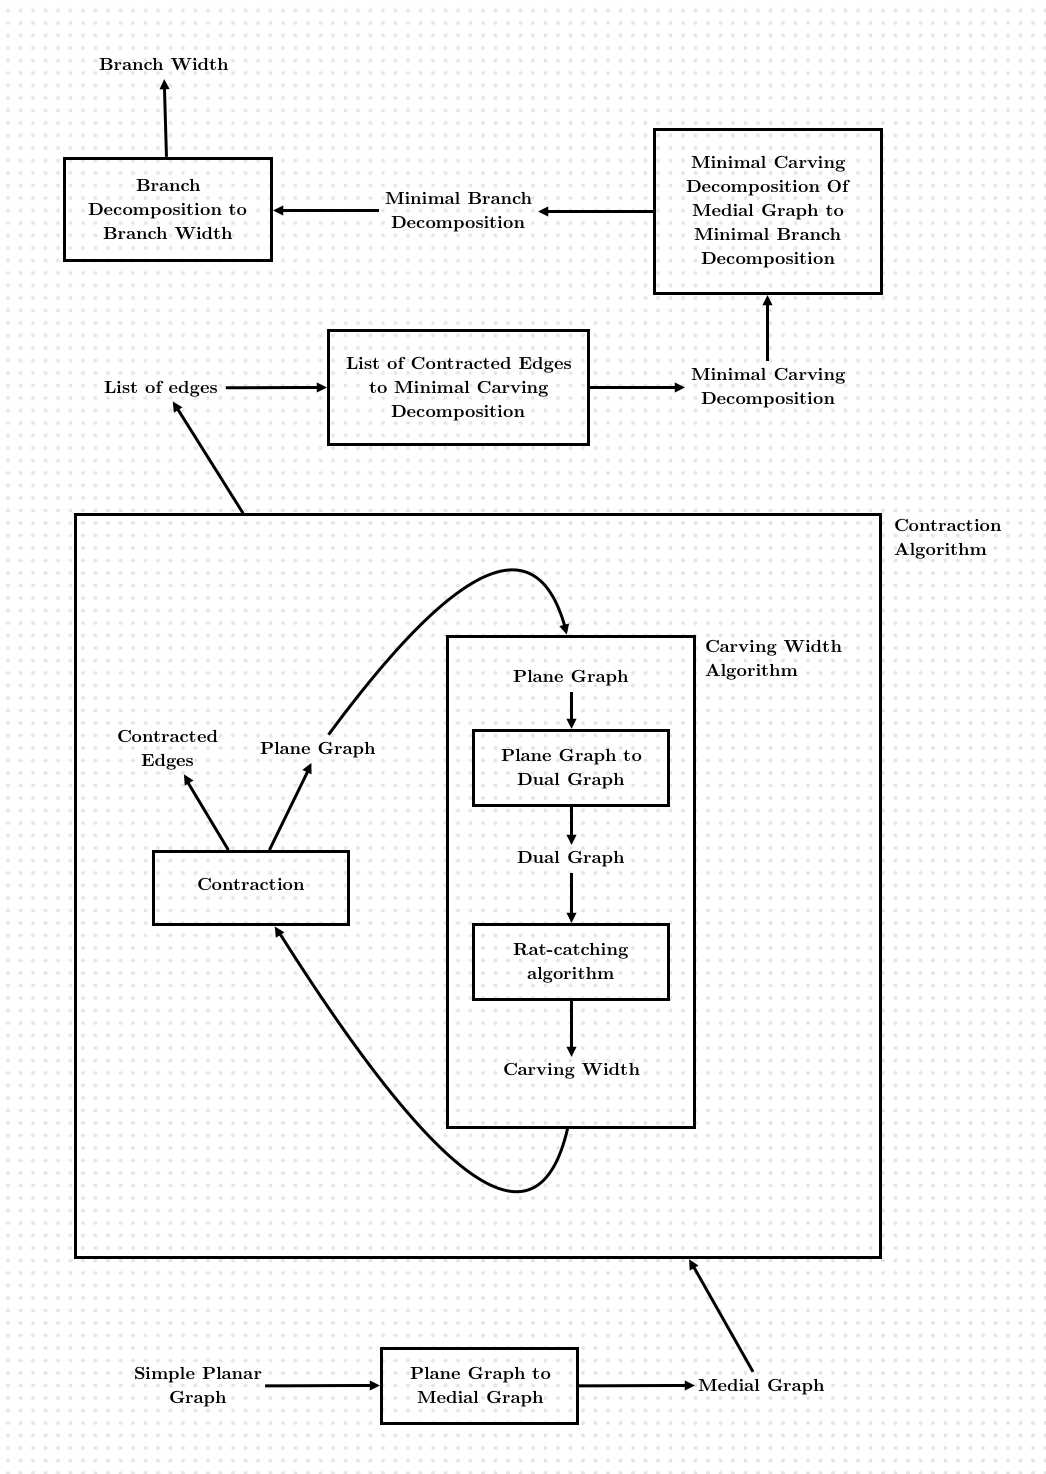
\includegraphics[width=\textwidth]{./images/overview.png}
		\caption{Overview of the algorithm}
		\label{fig:overview}
	\end{figure}

\section{Data Structures and implementation considerations}

	For many of the subroutines, the algorithm needs to deal with parallel edges and be able to tell them apart, therefore the implementation encodes a graph as an adjacency list of edges and a map from unique edge IDs its vertex-pair.

	I have chosen to assign IDs such that if one half-edge has ID $i$ then the other half-edge has ID $-i$, therefore the absolute value $|i|$ uniquely identifies an undirected edge.

	\pyfile{graph.py}{0}{33}

\section{The algorithm}

	The main computational problem of this paper is \textsc{The Planar Minimum Branch Decomposition Problem}.

	\begin{definition}\label{def:mbdp}
		\textsc{The Planar Minimum Branch Decomposition Problem}

		Input: Given a simple connected planar graph $G$.

		Output: A minimum branch decomposition of $G$.
	\end{definition}

	The algorithm described in this paper solves \textsc{The Planar Minimum Branch Decomposition Problem} in polynomial time.

	This section describes the algorithm given by Seymour and Thomas\cite{ST93} by identifying a set of practical problems and subproblems and how they relate.
	
	Problem \ref{def:mbdp} is the overarching problem. It can be broken down into many smaller subproblems.

	Considering a plane graph $G$, you can compute a minimum branch decomposition $(B_G, \delta_G)$ of $G$ from a minimum carving decomposition $(C_{G^\times}, \lambda_{G^\times})$ of the medial graph $G^\times$ of $G$.

	Therefore problem \ref{def:mbdp} breaks down into subproblems \ref{problem:medial}, \ref{problem:mcd} and \ref{problem:mcd-to-mbd}.

	\begin{problem}\label{problem:medial}
		Given a plane graph $G$, output a medial graph $G^\times$, along with a bijectional relation between medial nodes $V(G^\times)$ and edges $\mathbb{E}(G)$.
	\end{problem}

	\begin{problem}\label{problem:mcd}
		Given a plane graph $M$, output a minimum carving decomposition of $M$.
	\end{problem}

	\begin{problem}\label{problem:mcd-to-mbd}
		Given a minimum carving decomposition of a medial graph of $G$, output a minimum branch decomposition of $G$.
	\end{problem}

	With subroutines for all three problems, the implementation obtains a branch decomposition like so.

	\pyfile{branch_decomposition.py}{6}{22}

	Here are three sections, one for each subproblem.

	\subsection{Medial graph}

		Solving problem \ref{problem:medial}.

		Recall the definition \ref{def:medial}.

		I assume that the input graph $G$ is a rotation system. Given this format, any two consecutive edges $w$ and $v$ in some face of $G$ are therefore consecutive vertices in the neighborhood of the vertex $a$ that $w$ and $v$ share.

		\begin{figure}[H]
			\centering
			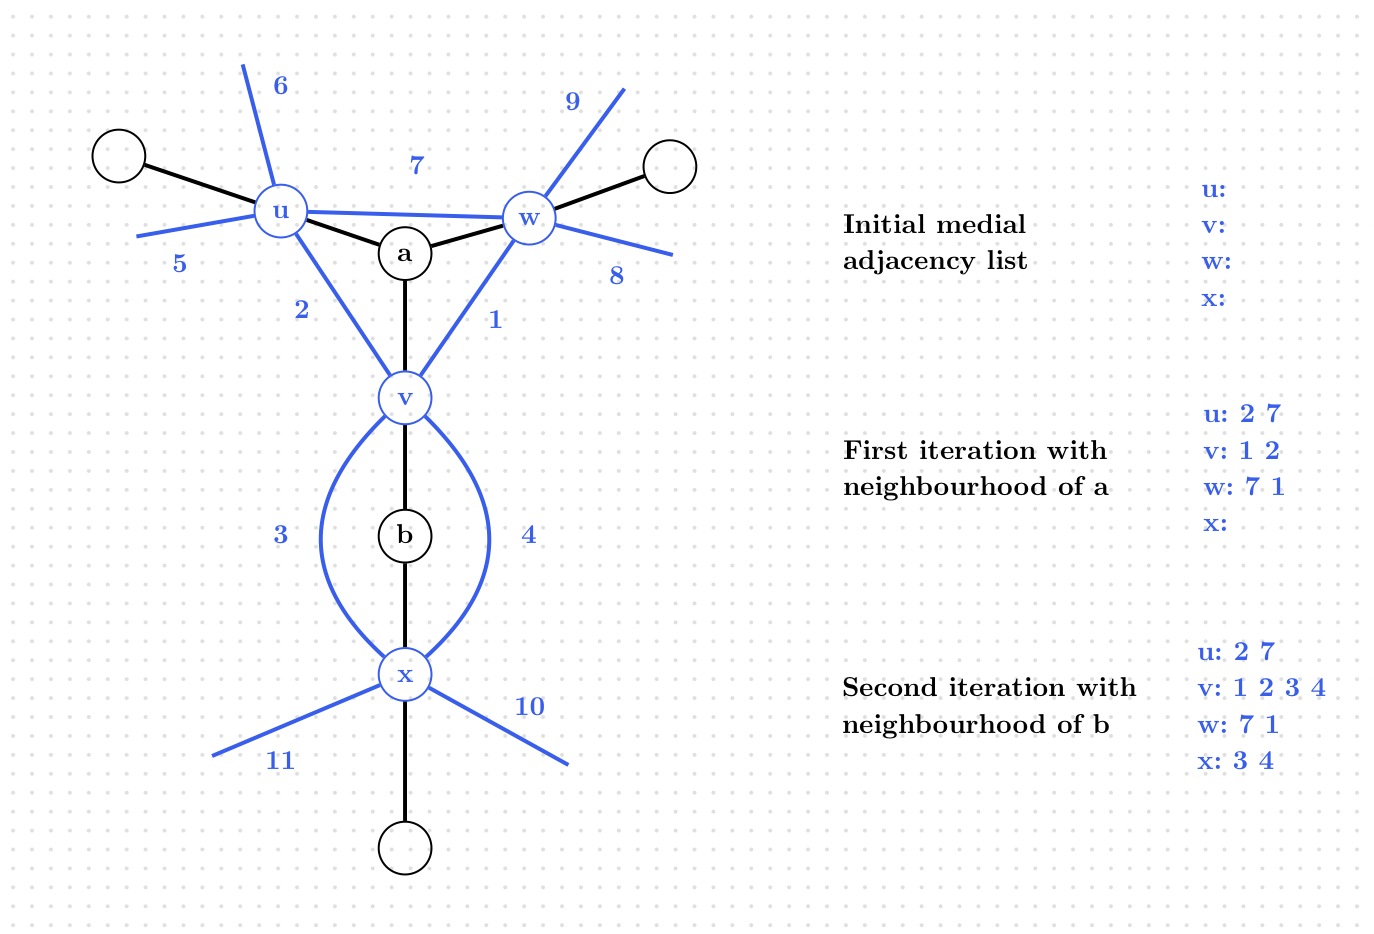
\includegraphics[width=\textwidth]{./images/medial-implementation-4-reg-argument.png}
			\caption{Two iterations of the algorithm computing a medial rotation system}
			\label{fig:overview}
		\end{figure}
		
		A medial graph is 4-regular; every node has degree 4. From the perspective of some medial node $v$, in some single iteration of the loop on line 14, two links are added to the neighborhood of $v$ in counterclockwise ordering, and later the two other links are added to the neighborhood of $v$ also in counterclockwise ordering. Therefore the medial graph $M$ is a rotation system.

		\pyfile{medial_graph.py}{5}{27}
	
	\subsection{Minimum Branch Decomposition from Minimum Carving Decomposition}

		Solving problem \ref{problem:mcd-to-mbd}.

		For both branch- and carving-decompositions, I have chosen a data structure of tuples of either more tuples or integers. This has a straightforward translation to the Newick Tree Format, a concise notation for tree structures.

		To then solve the above-mentioned problem, the implementation recursively returns either returns a copy of any tuple it encounters or returns a tuple of integers for any integer in encounters, using the relation node\_to\_vertexpair.

		This effectively replaces the leaf nodes of the carving decomposition with vertex-pairs for the branch decomposition.

		\pyfile{branch_decomposition.py}{5}{19}
			
	\subsection{Minimum Carving Decomposition}

		To solve \ref{problem:mcd} \ref{} gives a contraction algorithm.

		By doing a series of edge contractions on a graph $M$, where the carving width does not increase until 3 vertices remain, then the series of contracted edges along with the three vertices, can be assembled into a minimum carving decomposition of $M$.

		The implementation finds a nonincreasing contraction by doing a linear search over every edge.
		
		No consideration has yet been given to any potential clever orderings of the edges that might improve the running time.

		The "contraction" function, given a pair of vertices $u,v$, returns a new unique vertex ID $w$ (instead of reusing either $u$ or $v$), therefore by keeping track of which vertex is a contraction of which vertex-pair, in say a dictionary, constructing the decomposition is then a matter of recursively looking up vertices in the dictionary. Repeating this until only vertices of $M$ remain gives a carving decomposition in the aforementioned Newick-like nested tuple format.

		\pyfile{carving_decomposition.py}{7}{50}

		The contraction algorithm depends on a function to compute a contraction and a function to compute the carving width of a graph. This is problems \ref{problem:contraction} and \ref{problem:cw}.

		\begin{problem}\label{problem:contraction}
			Given a graph $M$ and a pair of vertices $\{u, v\}$, output the graph resulting from a contraction.
		\end{problem}

		\begin{problem}\label{problem:cw}
			Given a plane graph $M$ that might have parallel edges, output the carving width of $M$.
		\end{problem}

		\subsubsection{Contraction}

			Solving problem \ref{problem:contraction}.

			As the resulting graph is later given as an argument to functions assuming a rotation system of a planar graph, the implementation needs to preserve this invariant when contracting.

			Recall the definition \ref{def:contraction}. As this contraction removes all edges connecting a pair of vertices, the resulting graph will not exhibit any self-loops. I suspect reconciling this and the rotation system could be difficult, but in this context, it is irrelevant.

			For a contraction of vertices $a$ and $b$, I have chosen to create a new vertex ID $c$ (instead of, as the definition suggests, reusing either $a$ or $b$), as this makes the implementation, for assembling the carving decomposition, simpler.

			First, let any edges incident to $a$ or $b$ be incident to $c$ instead. Then creating the neighborhood of the new vertex $c$ is done by firstly finding any shared edge $e$; an edge that was in the neighborhood of both $a$ and $b$. This edge has some ID $e$ and the other half-edge, ID $-e$, will therefore be in the neighborhood of $b$. Now "rotating" the lists representing the neighborhoods of $a$ and $b$ such edge $e$ and $-e$ is at index 0, in their respective lists, means that a concatenation of the lists will preserve the clockwise ordering around the new vertex $c$. And finally, remove any edges connecting $a$ and $b$.
			
			This is where telling apart two edges that are parallel, by having edge IDs, becomes very useful. Inferring where to stitch together the neighborhoods to preserve the clockwise ordering, solely from an adjacency list, is way less practical.

			\pyfile{contraction.py}{4}{49}

		\subsubsection{Carving Width}

			Solving problem \ref{problem:cw}.

			The rat-catching algorithm decides whether $cw(M) \geq k$ with $k \in \mathbb{N}^+$. The boolean results of this algorithm for $k=\{1,2,3,...\}$ are monotonic, so you can perform a binary or linear search to find the smallest $k$ where $cw(M) \geq k$ is true.

			\pyfile{carving_width.py}{7}{8}
			\pyfile{carving_width.py}{132}{158}

	\section{The Rat-Catching Algorithm}

		The rat-catching algorithm decides $cw(M) \geq k$ with $k \in \mathbb{N}^+$.

		The rat-catching algorithm can be described as a game of two players, the rat and rat-catcher. Considering a graph $M$, the edges of a face can be thought of as walls of a room and vertices as the corners of some rooms. The rat moves from corner to corner along the walls and the rat-catcher moves from room to room through some wall. The rat-catcher can force the rat away from some walls by making noise. A round of this game is played with some noise level $k$. The rat-catcher wins the round if they can force the rat to be in some wall of the room that they are in, and the rat wins the round if there is a strategy whereby the rat can escape indefinitely.

		Additionally, if $\Delta(M) \geq k$ then the rat wins. The argument for why this is true is glossed over in \ref{BGZ15}. This is discussed in section \ref{}.

		So if $\Delta(M) < k$, then the game is played to determine an outcome, otherwise the rat is said to win.

		We have arrived at the crux of the algorithm. Does the rat win for some integer $k$?

		For some noise level and location of the rat-catcher, exactly which edges are noisy and which are quiet are definitions \ref{def:edge-quiet} and \ref{def:face-quiet}.

		\begin{definition}\label{def:edge-quiet}
			When the rat-catcher is on some edge $e_1$, then edge $e_2$ is noisy iff. there is a closed walk of length scrictly less than $k$ containing $e_1^*$ and $e_2^*$ in the dual $M^*$.
		\end{definition}

		An edge $e$ is called quiet iff. $e$ is not noisy.

		\begin{definition}\label{def:face-quiet}
			When the rat-catcher is in some face $f$, then edge $e$ is noisy iff. there is a closed walk of length scrictly less than $k$ containing $f^*$ and $e^*$ in the dual $M^*$.
		\end{definition}

		A quiet subgraph $Q(M, k, e)$, for some graph $M$, some noise level $k$ and some $e \in \mathbb{E}(M)$, is a subgraph of $M$ with the vertex set $V(Q(M, k, e)) = V(M)$ and the edge set

		$\mathbb{E}(Q(M, k, e)) = \{e_1 \st $ every closed walk of $M^*$ containing $e_1^*$ and $e_2^*$ has length at least $k\}$

		\begin{problem}\label{problem:noisy-subgraph}
			Given a plane graph $M$ that might have parallel edges, an edge $e \in \mathbb{E}(M)$, and noise level $k \in \mathbb{N}^+$, output the quiet subgraph $Q(M, k, e)$.
		\end{problem}

		Problem \ref{problem:noisy-subgraph} depends on a function for computing the dual of a graph. Computing a dual graph is problem \ref{problem:dual}.

		\begin{problem}\label{problem:dual}
			Given a plane graph $M = \{V, E\}$ that might have parallel edges, output the dual of $M$.
		\end{problem}

		The game states and possible moves, for some graph $M$ and some noise level $k$, can be described as a graph $H(M, k)$.

		Let $F(M)$ be the set of faces of $M$.

		Let $S$ be every possible state when the rat-catcher is in a face some of which might be losing states. $S = \{ (f, v) \st v \in V(M) \land f$ is a face of $ M \}$.

		Let $T$ be every possible state when the rat-catcher is on an edge. $T = \{ (e, C) \st e \in \mathbb{E}(M) \land C$ is a component of $Q(M, k, e) \}$.
		
		With the graph of possible moves $H$, the only missing piece of the rat-catching algorithm is how to determine the outcome.

		You can mark states/vertices of the graph $H$ that are losing states, and then repeatedly mark any state that leads to a losing state, until either every state is marked or no more states can be marked. If every state is marked then the rat-catcher wins, otherwise the rat wins.

		Solving problem \ref{problem:cw}.

		The vertices of the game state graph $H$ are initialized by computing the elements of $T$ and $S$, while edges of $H$ are not explicitly kept in any data structure, but instead checked while playing the game.

		Losing states (the tuples $(f,v) \in S$ where $v \in f$) are marked as losing.

		The outcome of the game is computed by marking states as losing.
		
		Considering a tuple $(e, C) \in T$, if all $(f, v)$ where $v \in V(C)$ is losing then $(e, C)$ is losing.

		Considering a tuple $(f, v)$, if there exists a tuple $(e, C)$ that is losing where $e \in f$ and $v \in V(C)$ then $(f, v)$ is losing.

		\pyfile{carving_width.py}{78}{130}

		\subsection{Quiet subgraph}

			Solving problem \ref{problem:noisy-subgraph}.

			Recall the definition \ref{def:edge-quiet}.

			Let $s_1$ and $t_1$ be the vertex-pair for the link $e_1^*$ and let $s_2$ and $t_2$ be the vertex-pair for the link $e_2^*$.

			\begin{claim}
				The shortest closed walk that includes both $e_1^*$ and $e_2^*$ is the minimum of either $$d(s_1, s_2) + d(t_1, t_2) + 2$$ or $$d(s_1, t_1) + d(s_2, t_2) + 2$$. Where $d(u, v)$ is the length of the shortest $u,v$-path.
			\end{claim}

			The single source shortest distances can then be computed using a breadth-first approach.

			Using the mapping from links to edges, and the fact that an edge $e$ is called quiet iff. $e$ is not noisy, the quiet edges can be obtained in the natural way.

			Computing the quiet subgraph and the components thereof is done with a depth-first search approach.

			The edges of the components are irrelevant for the rest of the algorithm, so only a list of vertices is returned for each component.

			\pyfile{carving_width.py}{10}{76}

		\subsection{Dual graph}\label{impl:dual}

			Solving problem \ref{problem:dual}

			No other path of the implementation needs the assumption that the dual is planar, therefore the output doesn't need to be a rotation system. This simplifies the implementation.

			The dual has a vertex for each face of the input graph. The faces are found by selecting an unmarked half-edge, then marking all the edges of the face it belongs to, and repeating this until all half-edges are marked.

			The next halfedge $e_{i+1}$ after the current halfedge $e_i = \{u, v\}$ is the edge just before $-e_i$ in the neighborhood list for vertex $v$.

			\pyfile{dual_graph.py}{4}{56}

\section{Results}

	The algorithm has been implemented in Python 3.12.2. The source code is available at \url{https://github.com/hojelse/thesis}.
	
	The implementation has been tested on a set of graphs, and the results are as expected. \todo{more}

	\todo{Agreement with Andreas' implementation on 6-100 vertices graphs, 10 different graphs}

	\todo{note Tested on cubic planar graph}

	\todo{tested by permuting vertex labels should not change the branch width}

	\todo{test that bw follows theoretical bound}

	Fomin and Thilikos 2006, New upper bound obn the decomposability pf planar graphs, bw <= 4.5 * sqrt(N) on planar

	Semour Thomas 1994, Call routing and ratcatcher, bw(G) = bw(dual(G)) assuming G is bridgeless planar graphs

	then the dual has half the vertices of the primal

	4.5 * sqrt(N/2)

	<=> 3.18199 * sqrt(n)

	Test bw <= 3.18199 * sqrt(N) on cubic planar graphs

	\todo{graphing theoretical bound}

\newpage
\section{References}
	\printbibliography

\newpage
\section{Appendix}
	% \pyfile{branch_decomposition.py}{0}{1000}
	% \pyfile{branch_width_brute_force.py}{0}{1000}	
	% \pyfile{branch_width.py}{0}{1000}
	% \pyfile{carving_decomposition.py}{0}{1000}
	% \pyfile{carving_width_brute_force.py}{0}{1000}
	% \pyfile{carving_width.py}{0}{1000}
	% \pyfile{contraction.py}{0}{1000}
	% \pyfile{dual_graph.py}{0}{1000}
	% \pyfile{Graph.py}{0}{1000}
	% \pyfile{medial_graph.py}{0}{1000}
	% \pyfile{parse_graph.py}{0}{1000}
	% \pyfile{parse_newick.py}{0}{1000}

\end{document}
